\chapter{Kieker Monitoring Component}\label{chap:components}


	\section{Configuration}

		\notify The monitoring part of \Kieker\ can easily configured and adjusted using the configuration file named \dir{\monitoringPropertiesFile}. By default, the configuration file within \dir{\monitoringJar} will be used. If a modified file should be used, the configuration file within \dir{\KiekerDir/META-INF} can be used as a base. To inform \Kieker\  about this, following parameter has to be add while calling the JVM:

		\setBashListing
		\begin{lstlisting} 
			-Dkieker.monitoring.properties=<ANY-DIR>/kieker.monitoring.properties      
		\end{lstlisting}

		A listing of all variables and their explanation can be found in the
		appendix.


	\section{Monitoring Records}

		As can be seen in the example chapter, the records are the objects which store the monitored informations somehow. To be more precisely, they are not really part of \KiekerMonitoringPart\, but in order to use them in this chapter, they will be examined now.\\ To implement an own record, the easiest way is to extend the already existing abstract class \class{kieker.common.record.AbstractMonitoringRecord}. The implementation of a record has to provide methods to put the whole content of the record into an array (of Object) so that the other components of \Kieker\  are able to persist the data. Due to the fact that the data has to be read again, the records have to provide methods to restore the content from an array as well. Listing \ref{listing:MyRecord} shows a simple record implementation which stores informations about the called class and method.

		\setJavaCodeListing
		\lstinputlisting[caption=MyRecord.java, label=listing:MyRecord]{\customComponentsBookstoreApplicationDir/src/bookstoreTracing/MyRecord.java}


	\section{Monitoring Probes}

		The probes are responsible for the monitoring itself. They decide which (and where) informations should be collected. Technically they were already used in the example chapter by surrounding the method calls with the correct statements to clock, to produce the records and to deliver these records to the monitoring controller.

		% Make sure that this listing will be modified, once the sourcecode changes!!!
		% It must show the whole monitoring of the bookstorecall, from getting the first time to persisting of the record!!
		\lstinputlisting[firstline=20, lastline=29, caption=Cutting from Bookstore.java, label=listing:cuttingBookstore]{\manualInstrumentedBookstoreApplicationDir/src/bookstoreApplication/Bookstore.java}

		Other specific probes could for example record only the amount of delivered bytes between methods or record only every second method call as well. The possibility to use annotations to make the monitoring much more comfortable will be shown in the appendix.

	\section{Monitoring Log Writers}

		The so called monitoring log writers serialize and persist the recorded informations into files, databases and so on. In other words: They get an instance of an \class{IMonitoringRecord} and produce and output of any nature whatsoever.\\
		Some writers are already implemented, as can be seen in their hierarchy in Figure \ref{figure:monitoringLogWritersHierarchy}.

		% This is the diagram with the hierarchy of the writers.
		\begin{figure}[H]
			\begin{centering}
				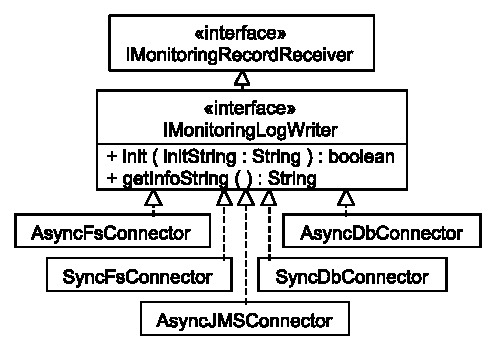
\includegraphics[width=0.5\textwidth]{images/kieker_writerimpls}
				\caption{The inheritance hierarchy of the current implemented monitoring log writers}
				\label{figure:monitoringLogWritersHierarchy}
			\end{centering}
		\end{figure}


		As the example chapter already showed it, every monitoring record is sent to the \class{MonitoringController} which itself calls the current writer. The writer uses normally the \method{toArray()} method of the record to get the stored informations from the record as handable array. The writer writes these objects for example into a file.\\
		The implementation of an own writer is quite simple and can be done by implementing the interface \class{kieker.monitoring.writer.IMonitoringLogWriter}. Listing \ref{listing:MyWriter} shows an example writer which uses a named pipe to write the given records directly into the memory. The class \class{MyPipe} is descriped in the appendix of the tutorial. 

		\setJavaCodeListing
		\lstinputlisting[caption=MyWriter.java, label=listing:MyWriter]{\customComponentsBookstoreApplicationDir/src/bookstoreTracing/MyWriter.java}

		Making sure that \Kieker\  uses the new writer is done by modifying the above mentioned configuration file \dir{\monitoringPropertiesFile}.

		\setBashListing       
		\begin{lstlisting}
			monitoringDataWriter=bookstoreTracing.MyWriter
			monitoringDataWriterInitString=somePipe
		\end{lstlisting}

		The first property decides which writer should be used. If none of the already implemented writers is used, the whole name of the class of the writer has to be delivered. The second property is an init string which can be used to initialize the writer in any way. In this case the parameter is used to tell the writer the name of the pipe to be used.\\
		\warning It is important that every implemented writer class has a corresponding reader class, so that the persisted data can be loaded again.